\documentclass[12pt]{article}
\usepackage{lmodern}
%\usepackage[utf8]{vietnam}
\usepackage{amsmath}
\usepackage{amsfonts}
\usepackage{indentfirst}
\usepackage{fancyhdr}
\usepackage{graphicx}
\usepackage{xcolor}
\usepackage{listings}
\usepackage{multicol}
\usepackage{titletoc}
\usepackage{tikz}
\usetikzlibrary{calc}
\usepackage{background}
\newcommand\DeactivateBG{\backgroundsetup{contents={}}}
\renewcommand\ActivateBG{\backgroundsetup{scale=2,angle=0,firstpage=false,opacity=0.2,
contents={\begin{tikzpicture}[remember picture,overlay]
\node at ([yshift=0pt, xshift=0pt]current page.center){\includegraphics[]{Logo/logoUCPC.png}}
\end{tikzpicture}}}}
\tikzset{axis line style/.style={thin, gray, -stealth}}
\usepackage{geometry}
\geometry{
	a4paper,
	left = 20mm,https://www.overleaf.com/project/6290fe5cb8b57786becc2396
	right = 20mm,
}

%\usepackage{afterpage}






\usepackage{fancyhdr}
\pagestyle{fancy}

\usepackage{afterpage}

\newcommand\blankpage{%
    \null
    \thispagestyle{empty}%
    \addtocounter{page}{-1}%
    \newpage}


\lstset{language=C++,
	numbers = left,
	language=C++,
    basicstyle=\ttfamily,
    keywordstyle=\color{blue}\ttfamily,
    stringstyle=\color{red}\ttfamily,
    commentstyle=\color{green}\ttfamily,
    morecomment=[l][\color{magenta}]{\#}
	columns=fullflexible,
	tabsize=2,
}

\everymath{\displaystyle}
\renewcommand{\familydefault}{lmss}
\lhead{University of Information Technology, VNU-HCM \\ UIT Collegiate Programming Contest 2022}

\rhead{}


\renewcommand{\thesection}{Problem \Alph{section}: }
\renewcommand*{\contentsname}{\hfill List of problems \hfill}
\titlecontents{section}[2.3em]
{\smallskip}
{\hspace{1 cm} \fontsize{16}{16} \bfseries{\thecontentslabel} \hspace{0.5 cm} \MakeUppercase}
%{\hspace{1 cm} \fontsize{16}{16} \bfseries{\thecontentslabel} \enspace \MakeUppercase}
{\hspace*{-5.3em}}
{\hfill}

\begin{document}
    \DeactivateBG{}
    \begin{titlepage}
    \begin{center}
    % \includegraphics[height = 20mm]{Logo/1.png}
    % \includegraphics[height = 20mm]{Logo/2.png}
    % \includegraphics[height = 20mm]{Logo/3.png}
    % \includegraphics[height = 20mm]{Logo/4a.png}
    
    
    \vspace*{3\baselineskip}
    \fontsize{20}{20}\textbf{UIT COLLEGIATE PROGRAMMING CONTEST}
    \vspace*{2\baselineskip}
    
    \textbf{May 29, 2022}
    
    \vspace*{2\baselineskip}
    \includegraphics[height = 20mm]{Logo/1.png}
    \includegraphics[height = 20mm]{Logo/2.png}
    \includegraphics[height = 20mm]{Logo/3.png}
    \includegraphics[height = 20mm]{Logo/4a.png}
    
    \end{center}
    \tableofcontents
    %\afterpage{\null\thispagestyle{empty}\newpage}
    \afterpage{\blankpage}
\end{titlepage}
    \pagebreak
    \ActivateBG{}
	\section{Simple Chess}
	
	\vspace{-0.5cm}
	\begin{table}[!h]
		\hspace{1cm}
		\begin{tabular}{ll}
			Time limit  &:  1s        \\
			Memory limit &:  256MB         \
		\end{tabular}
	\end{table}
	
	Given two $4 \times 4$ chess boards with pawns on the board, each piece can move forward, upward, right, left exactly $1$ square, and cannot be captured by any other pieces (also the pawn won't be promoted to any other pieces when it reach the end of the board).
	
	Given the state of each board, you have to calculate the minimum number of moves required to transform from the first chessboard to the second chessboard. The picture below shows the transformation from the first board to the second board.
	
	\begin{center}
		\includegraphics[width = 150mm]{example.png}
		
		The minimum number of moves required to make the first chessboard become the second chessboard in the example is $4$.
	\end{center}
	
	\subsection*{Input}
	
	Input consists of two $4 \times 4$ matrices.
	
	The first $4$ lines represent the state of the first chessboard. Let the state of the first table is $a_{i,j}$ $(1 \le i,j \le 4)$, $a_{ij}$ = 1 means that there is a pawn on the $i$-th row $j$-th column, $a_{ij} = 0$ means that the square from $i$-th row $j$-th column is empty.
	
	The following $4$ lines represent the state of the second chessboard, with same meaning as the first one.

	\subsection*{Output}
	
	Print a single non-negative integer, the minimum number of moves required to make the first chessboard become the second chessboard.
	
	\begin{center}
		\begin{tabular}{|p{6cm}|p{6cm}|}
			\hline
			\textbf{Sample Input} &
			\textbf{Sample Output} \\
			\hline
			{\fontfamily{qcr}\selectfont 1 0 0 0} & {\fontfamily{qcr}\selectfont 4} \\
			{\fontfamily{qcr}\selectfont 0 0 1 0} & \\
			{\fontfamily{qcr}\selectfont 0 0 0 1} & \\
			{\fontfamily{qcr}\selectfont 0 1 0 0} & \\
			{\fontfamily{qcr}\selectfont 0 1 0 0} & \\
			{\fontfamily{qcr}\selectfont 0 0 0 0} & \\
			{\fontfamily{qcr}\selectfont 0 0 1 0} & \\
			{\fontfamily{qcr}\selectfont 1 0 0 1} & \\
			\hline
		\end{tabular}
	\end{center}
	\endpage
	%\afterpage{\null\thispagestyle{empty}\newpage}
	\afterpage{\blankpage}
	%\newb
	\section{The sound of a cat}
	
	\vspace{-0.5cm}
	\begin{table}[!h]
		\hspace{1cm}
		\begin{tabular}{ll}
			Time limit  &:  2s        \\
			Memory limit &:  256MB        \\
		\end{tabular}
	\end{table}
	
	WooZi has a cat named Mimi which looks like this:
	
	\begin{center}
		\includegraphics[height = 75mm]{cat.png}
	\end{center}
	
	Mimi usually makes 3 sounds as follow:
	
	
	\begin{itemize}
	
	\item {\fontfamily{qcr}\selectfont meow}: This sound starts with one character {\fontfamily{qcr}\selectfont m}, followed by at least 1 character {\fontfamily{qcr}\selectfont e}, then continues followed by one character {\fontfamily{qcr}\selectfont o}, and ends with at least one character {\fontfamily{qcr}\selectfont w}.
	\item {\fontfamily{qcr}\selectfont purr}: This sound starts with two characters {\fontfamily{qcr}\selectfont pu}, followed by at least two characters {\fontfamily{qcr}\selectfont r}.
	\item {\fontfamily{qcr}\selectfont roar}: This sound starts with one character {\fontfamily{qcr}\selectfont r}, followed by at least one character {\fontfamily{qcr}\selectfont o}, and ends with two characters {\fontfamily{qcr}\selectfont ar}.
	
	\end{itemize}
	
	Help WooZi distinguish those types of sounds!

	
	\subsection*{Input}
	
	The first line contains a positive integer $t$ $(1 \le t \le 100)$ as the number of sounds that Mimi had made.
	
	Each of the next $t$ lines contains a string $s$ of no more than $30$ characters, consisting of only lowercase English letters.
	
	\subsection*{Output}
	
	Output includes $t$ lines, each contains the types of sounds that Mimi had made. If it does not fall into one of these three types of sounds, print {\fontfamily{qcr}\selectfont human noises}.	
	
	\begin{center}
		\begin{tabular}{|p{6cm}|p{6cm}|}
			\hline
			\textbf{Sample Input} &
			\textbf{Sample Output} \\
			\hline
			{\fontfamily{qcr}\selectfont10} &  {\fontfamily{qcr}\selectfont meow} \\
			{\fontfamily{qcr}\selectfont meeeeowwwwwwwww} & {\fontfamily{qcr}\selectfont purr} \\
			{\fontfamily{qcr}\selectfont purrrrrrrrr} & {\fontfamily{qcr}\selectfont human noises} \\
			{\fontfamily{qcr}\selectfont puuurr} & {\fontfamily{qcr}\selectfont meow} \\
			{\fontfamily{qcr}\selectfont meowwwwww} & {\fontfamily{qcr}\selectfont human noises} \\
			{\fontfamily{qcr}\selectfont roooooaar} & {\fontfamily{qcr}\selectfont roar} \\
			{\fontfamily{qcr}\selectfont  roooooooooooooar} & {\fontfamily{qcr}\selectfont human noises} \\
			{\fontfamily{qcr}\selectfont  hello} & {\fontfamily{qcr}\selectfont human noises} \\
			{\fontfamily{qcr}\selectfont  ppuurr} & {\fontfamily{qcr}\selectfont human noises} \\
			{\fontfamily{qcr}\selectfont mmmmmeow} & {\fontfamily{qcr}\selectfont human noises} \\
			{\fontfamily{qcr}\selectfont rroar} & \\
			\hline
		\end{tabular}
	\end{center}
	
	\pagebreak
	
    \section{A great invention}
	
	\vspace{-0.5cm}
	\begin{table}[!h]
		\hspace{1cm}
		\begin{tabular}{ll}
			Time limit  &:  1s       \\
			Memory limit &:  256MB         \
		\end{tabular}
	\end{table}
	
	As everybody knows, the \textbf{Homo sapiens} have a great history. They discovered nature, passed the ocean and explored the space. Moreover, electricity is created, powerful mechanics are designed due to the intelligence of the humans. However, these results could not be done easily, or would never happen, if they had not published a great invention, called \textbf{Mathematics}.
	
	It is very easy for everyone to recognize the strong application of Mathematics. It could be used to calculate the weight of various things, to find the height of the buildings or to evaluate the probabilities. Moreover, Mathematics is the foundation of science and technology, which plays an important role in the Modern Age. If Mathematics was not invented, there would not be The Great Wall, or The Golden Gate Bridge. As a result, Mathematics is a very important subject, taught from elementary level to postgraduate in almost countries.
	
	Today, Stephen has gone to lecture on Discrete Structures, with focus on Arithmetic and its application. The professor is giving a topic about the divisors of a number. Stephen just has been back to the college after traveling among the multiverse (and saved the world, for sure),  so he has misunderstood what the lecturer said. Unluckily, life is never like a dream, the professor let him go to the board.
	
	Let us review the definition of a divisor: a positive integer $b$ is said to be a divisor of a positive integer $a$ if and only if there exists a positive integer $k$ so that $a = bk$. For example, $2,5$ are two divisors of $20$.
	
	Let $f(i)$ be the sum of all divisors of $i$. For instance, $f(4) = 1 + 2 + 4 = 7$.
	
	The problem which is given to Stephen is after receiving a positive he needs to calculate the sum of $f(i)$ for all integers from $1$ to $n$, in other words $\sum_{i = 1}^{n}f(i)$. You should help him to calculate this value, if not, he will get zero for the processing mark, or have to retake this subject again.
	
	\subsection*{Input}
	
	Input consists of only one positive integer $n$ $( 1 \leq n \leq 10^{12})$, the number given by the professor.
	
	\subsection*{Output}
	
	A single integer, the answer for Stephen's problem, after getting the modulo for $10^9+7$.
	
	\begin{center}
		\begin{tabular}{|p{6cm}|p{6cm}|}
			\hline
			\textbf{Sample Input} &
			\textbf{Sample Output} \\
			\hline
			{\fontfamily{qcr}\selectfont 5} & {\fontfamily{qcr}\selectfont 21} \\
			\hline
		\end{tabular}
	\end{center}
	%\afterpage{\null\thispagestyle{empty}\newpage}
	%\pagebreak
	\afterpage{\blankpage}
	
	\section{Wizarding World}
	
	\vspace{-0.5cm}
	\begin{table}[!h]
		\hspace{1cm}
		\begin{tabular}{ll}
			Time limit  &:  1s        \\
			Memory limit &:  256MB         \
		\end{tabular}
	\end{table}
	
	  In Wizarding world, A Hogwarts’ school year is coming to an end. Harry and Ron have to perform well in locomotion charm – an incantation used to affect the movement of the target of the spell, in the final exam. Thus, they make a decision to play a game by using locomotion charm so as to improve their magical skills.\\
      In this game, the Wizarding world is regarded as a 2-dimension coordinate system. Howarts school has a circular shape with the centre at the coordinaters’ origin and the radius $d$. A ball is initially put in the position $(x, y)$. In each turn, Harry or Ron must move the ball by a translation vector which is selected in the pre-selected vectors. Also each player can once per game symmetrically reflect the ball relatively to the line $y=x$. Ron and Harry take turns, Ron goes first. A player who moves the ball to the outside of Howarts school loses.\\
      Help them to determine the winner in case of both play the game optimally.
	\subsection*{Input}
	
	The first line of the input contains 4 integers $x, y, n, d$ $(-200 \le x, y \le 200, 1 \le d \le 200, 1 \le n \le 20)$ - the initial coordinates of the ball, the radius $d$ and the number of vectors. It is guaranteed that the initial ball is in Hogwarts school. The following $n$ lines each contains two non-negative numbers $x_i$ and $y_i$ $(0 \le x_i, y_i \le 200)$ - the coordinates of the i-th vector. It is guaranteed that all the vectors are nonzero and different. 
	
	\subsection*{Output}
	
	You should print "Ron", if the winner is Ron, and "Harry" otherwise.
	
	\begin{center}
		\begin{tabular}{|p{6cm}|p{6cm}|}
			\hline
			\textbf{Sample Input 1} &
			\textbf{Sample Output 1} \\
			\hline
			{\fontfamily{qcr}\selectfont 0 0 2 3} & {\fontfamily{qcr}\selectfont Ron} \\
			{\fontfamily{qcr}\selectfont 1 1} & \\
			{\fontfamily{qcr}\selectfont 1 2} & \\
			\hline
		\end{tabular}
	\end{center}
	
	\begin{center}
		\begin{tabular}{|p{6cm}|p{6cm}|}
			\hline
			\textbf{Sample Input 2} &
			\textbf{Sample Output 2} \\
			\hline
			{\fontfamily{qcr}\selectfont 0 0 2 4} & {\fontfamily{qcr}\selectfont Harry} \\
			{\fontfamily{qcr}\selectfont 1 1} & \\
			{\fontfamily{qcr}\selectfont 1 2} & \\
			\hline
		\end{tabular}
	\end{center}
	
	\textbf{Note:} In the first test, Ron goes to the vector $(1;2)$, and Harry loses. In the second test Harry with his first move shifts the ball so that its coordinates are $(2;3)$, and Ron loses, as Ron has the only possible move — to reflect relatively to the line $y=x$. Harry will respond to it with the same move and return the ball in position $(2;3)$.
	
	%\afterpage{\null\thispagestyle{empty}\newpage}
	\afterpage{\blankpage}
	
	\section{A very hard problem}
	
	\vspace{-0.5cm}
	\begin{table}[!h]
		\hspace{1cm}
		\begin{tabular}{ll}
			Time limit  &:  1s        \\
			Memory limit &:  256MB         \\
		\end{tabular}
	\end{table}
	
	You are the best attendants who participate in the UIT Collegiate Programming Contest. So that, this problem is prepared as a relaxation. We strongly believe you can solve that easily.
	
	You are given a non-negative array $a$, which has $n$ elements, the $i$-th is called $a_i$, come up with two integers $l$ and $r$ $(1 \le l \le r \le n)$. Moreover, there are four types of queries:
	
	\begin{itemize}
		\item {\fontfamily{qcr}\selectfont \textbf{1 t x}}: Count the number of positions $i$, $(1 \le i \le n)$ so that $a_i \& t = x$. It is guaranteed that $t \& x = x$
		\item {\fontfamily{qcr}\selectfont \textbf{2 t x}}: Count the number of positions $i$, $(1 \le i \le n)$ so that $a_i | t = x$. It is guaranteed that $t | x = x$
		\item {\fontfamily{qcr}\selectfont \textbf{3 u v}}: Let $g(k)$ be the number of set $(j_1,j_2,\dots,j_k)$ so that:
		\begin{enumerate}
			\item $1 \le j_1 < j_2 < \dots < j_k \le n$
			\item $u \le a_{j_1} \& a_{j_2} \& \dots \& a_{j_k} \le v$
		\end{enumerate}
		
		You need to calculate the sum of $g(k)$ for all $l \le k \le r$ after getting the modulo for $10^9+7$.
		
		\item {\fontfamily{qcr}\selectfont \textbf{4 u v}}: Let $h(k)$ be the number of set $(j_1,j_2,\dots,j_k)$ so that:
		\begin{enumerate}
			\item $1 \le j_1 < j_2 < \dots < j_k \le n$
			\item $u \le a_{j_1} | a_{j_2} | \dots | a_{j_k} \le v$
		\end{enumerate}
		
		You need to calculate the sum of $h(k)$ for all $l \le k \le r$ after getting the modulo for $10^9+7$.
		
	\end{itemize}
	
	\textbf{Remind that:}
	
	\begin{itemize}
		\item Operator AND (written as $\&$) of two non-negative numbers $x$ and $y$ is an integer $z$, which its $i$-th bit is $1$ if and only if the $i$-th bit of both $x$ and $y$ is $1$, is $0$ otherwise.
		\item Operator OR (written as $|$) of two non-negative numbers $x$ and $y$ is an integer $z$, which its $i$-th bit is $1$ if at least one of two integers $x,y$ has $1$ in $i$-th bit, is $0$ otherwise.
	\end{itemize}
	
	Because this problem is a present from the setters, so you should complete all the queries, if you don't, we will be very sad.
	
	\subsection*{Input}
	
	The very first line of the input contains four positive integers $n,q,l,r$ $(1 \le l \le r \le  n \le 10^6; 1 \le q \le 10^6)$.
	
	The second line contains $n$ integers, $a_1,a_2,\dots,a_n$, the elements of array $a$ $(0 \le a_i < 2^{20})$.
	
	Next $q$ lines, each line contains for integers, describes a query as mentioned above. Every number given in queries is non-negative and less than $2^{20}$.
	
	It is guaranteed that the number of queries type {\fontfamily{qcr}\selectfont 1} and {\fontfamily{qcr}\selectfont2}, in sum, will not exceed $5 \times 10^3$.
	
	\subsection*{Output}
	
	For each query, a non-negative number should be printed, which is the answer of that query.
	
	\begin{center}
		\begin{tabular}{|p{6cm}|p{6cm}|}
			\hline
			\textbf{Sample Input} &
			\textbf{Sample Output} \\
			\hline
			{\fontfamily{qcr}\selectfont 4 4 1 2} & {\fontfamily{qcr}\selectfont 2} \\
			{\fontfamily{qcr}\selectfont 2 3 5 6} & {\fontfamily{qcr}\selectfont 2} \\
			{\fontfamily{qcr}\selectfont 1 3 2} & {\fontfamily{qcr}\selectfont 5} \\
			{\fontfamily{qcr}\selectfont 2 1 3} & {\fontfamily{qcr}\selectfont 3} \\
			{\fontfamily{qcr}\selectfont 3 1 2} & \\
			{\fontfamily{qcr}\selectfont 4 0 4} & \\
			\hline
		\end{tabular}
	\end{center}
	
	\pagebreak
	
	\section{Massive Mission}
	
	\vspace{-0.5cm}
	\begin{table}[!h]
		\hspace{1cm}
		\begin{tabular}{ll}
			Time limit   &:  1s        \\
			Memory limit &:  256MB         \\
		\end{tabular}
	\end{table}
	
	After several days being repelled by the Galicia-Volyn Army, the Red Special Forces had decided to change their military strategy. Aerial bombing was chosen and the location will be the K-Complex. As a result,  an investigation was held and some important information was collected.
	
	Suppose that we are considering the map of the K-Complex on the 2D space. The K-Complex consists of $n$ rectangular buildings. Each one is described by five integers $x,y,w,h$ and $\phi$. Two numbers $x$ and $y$ are coordinates of the building center on the 2D map, $w$ and $h$ one-by-one are its width and height, $\phi$, in degree, is the angle between the height axis of the building to the $Oy$ axis.
	
	To protect the K-Complex, the Galicia-Volyn Army has built The Great Hull, which includes several walls. The walls are surrounding the buildings of K-Complex and are built to minimize the area it is covered in. As a result, the shape of The Great Hull is a Convex Hull (that's why it has 'Hull' in its name).
	
\begin{center}
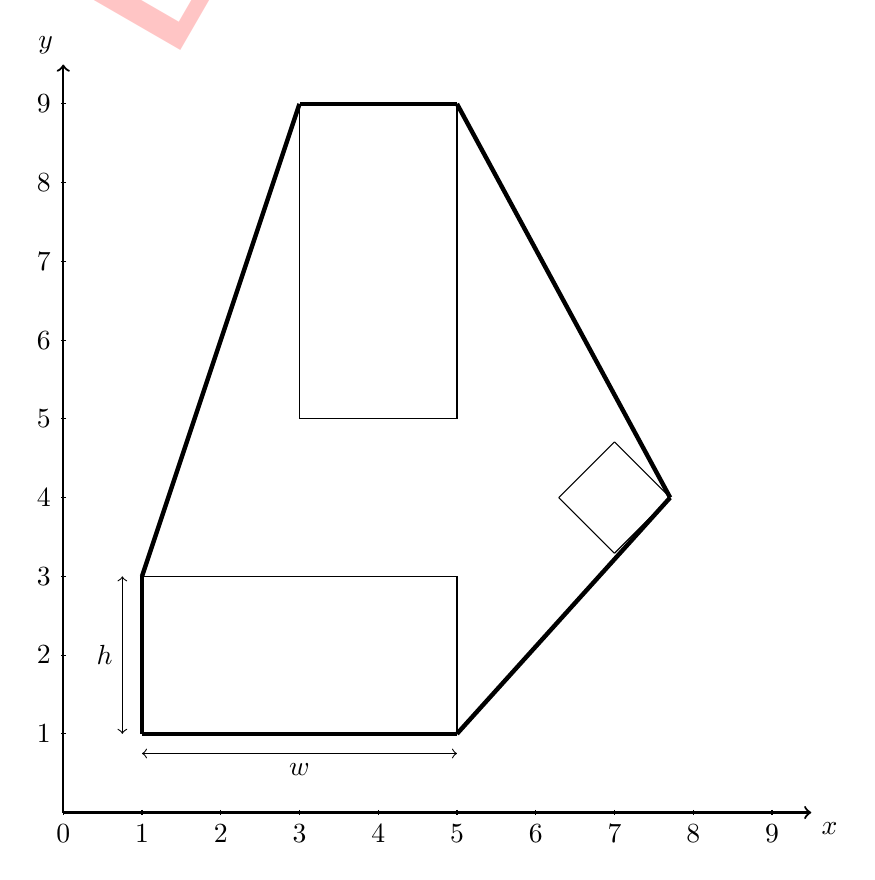
\begin{tikzpicture}[scale=1]
	% Draw axes
	\draw[thick,->] (0,0) -- (9.5,0) node[anchor=north west] {$x$};
	\draw[thick,->] (0,0) -- (0,9.5) node[anchor=south east] {$y$};
	\foreach \x in {0,1,...,9}
	\draw (\x cm,1pt) -- (\x cm,-1pt) node[anchor=north] {$\x$};
	\foreach \y in {1,2,...,9}
	\draw (1pt,\y cm) -- (-1pt,\y cm) node[anchor=east] {$\y$};
	\draw (1,1) -- (5,1);
	\draw (1,1) -- (1,3);
	\draw (1,3) -- (5,3);
	\draw (5,3) -- (5,1);
	\draw (3,5) -- (5,5);
	\draw (5,5) -- (5,9);
	\draw (5,9) -- (3,9);
	\draw (3,9) -- (3,5);
	\draw (6.2929,4) -- (7,3.2929);
	\draw (7,3.2929) -- (7.7071,4);
	\draw (7.7071,4) -- (7,4.7071);
	\draw (7,4.7071) -- (6.2929,4);
	\draw [ultra thick] (1,1) -- (5,1);
	\draw [ultra thick] (5,1) -- (7.7071,4);
	\draw [ultra thick] (7.7071,4) -- (5,9);
	\draw [ultra thick] (5,9) -- (3,9);
	\draw [ultra thick] (3,9) -- (1,3);
	\draw [ultra thick] (1,3) -- (1,1);
	\draw [<->] (0.75,1) -- (0.75,3)node[anchor = east, pos = 0.5] {$h$};
	\draw [<->] (1,0.75) -- (5,0.75)node[anchor = north, pos = 0.5]{$w$};
\end{tikzpicture}
\end{center}
	
	The area which inside The Great Hull is consider the part of The K-Complex and otherwise. Moreover, to make the bombing campaign more preciously, Hien, the commander of the Red Special Forces wants to know the percentage of space occupied by the buildings to the total space of the K-Complex.
	
	\subsection*{Input}
	
	The very first line of the input contains an integer $t$ $(1 \le t \le 10)$, the number of test cases.
	
	Each test case starts with an integer $n$ $(1 \le n \le 600)$, the number of buildings in the K-Complex. For each building, five integers $x,y,w,h,\phi$ $(0 \le x,y,w,h \le 10^4, -90 \le \phi \le 90)$ are given as described above. Remember that $\phi$ is given in degrees. It is guaranteed that the buildings will not be overlapped.
	
	\subsection*{Output}
	
	For each test case, print a single real number $p$ in a single line, the percentage of space occupied by the buildings to the total space of the K-Complex, with exactly two numbers after the decimal point.
	
	\begin{center}
		\begin{tabular}{|p{6cm}|p{6cm}|}
			\hline
			\textbf{Sample Input} &\textbf{Sample Output} \\ 
			\hline
			{\fontfamily{qcr}\selectfont 1} & {\fontfamily{qcr}\selectfont 46.16} \\
			{\fontfamily{qcr}\selectfont 3} & \\
			{\fontfamily{qcr}\selectfont 3 2 4 2 0} & \\
			{\fontfamily{qcr}\selectfont 4 7 4 2 90} & \\
			{\fontfamily{qcr}\selectfont 7 4 1 1 45} & \\
			\hline
		\end{tabular}
	\end{center}
	
	\textbf{Note:} The sample input is the case which is illustrated in the problem statement above.
	
	\pagebreak
	
	\section{Database}
	
	\vspace{-0.5cm}
	\begin{table}[!h]
		\hspace{1cm}
		\begin{tabular}{ll}
			Time limit   &: 1s        \\
			Memory limit &: 1024MB       \\
		\end{tabular}\\
	\end{table}
		
	In the University of Information Technology, there is a subject which makes the students feel very excited, called Database. To pass the final exam of this subject, a group of students in UIT has decided to make a project called \textbf{String Database}. This database works as follow:
	
	At first, there is only one string $s_0$.
	
	There are three types of queries that applied in this database:
	
	\begin{itemize}
		\item {\fontfamily{qcr}\selectfont \textbf{1 p n c}}: Create a new string $z$ with length $p$ by appending first $p-1$ characters of string $x$ - the $n$-th string in the Database and character $c$. For example, let $x =$ {\fontfamily{qcr}\selectfont abcd}, $p = 3$ and $c =$ {\fontfamily{qcr}\selectfont e}, $z$ will be {\fontfamily{qcr}\selectfont abe}. Then push $z$ into the back of the \textbf{String Database}.
		\item {\fontfamily{qcr}\selectfont \textbf{2 p n}}: Create a new string $z$ with length $p$ by appending first $p$ characters of string $x$ - the $n$-th string in the Database.  Then push $z$ into the back of the \textbf {String Database}.
		\item {\fontfamily{qcr}\selectfont \textbf{3 l r s}}: If from the index $l$-th to $r$-th string, inclusive, from the Database exists string $u$ so that string $s$ is a prefix of $u$, print \textbf{{\fontfamily{qcr}\selectfont yes}}, print \textbf{{\fontfamily{qcr}\selectfont no}} otherwise.
	\end{itemize}
	
	
	
	\subsection*{Input}
	
	The very first line of the input contains the string $s_0$, the only initial string of the \textbf{String Database} $(1 \le |s_0| \le 10^5)$.
	
	The second line of the input contains a non-negative integer $q$, denoting the number of queries $(1 \le q \le 3 \times 10^5)$.
	
	Next $q$ lines, each line stores a query which format is as mentioned above.
	
	Let there are $k$ strings in the database after performing first $i-1$ queries and the string in position $j$ is is $s_j$. Suppose that we are consider the $i $-th query, it is ensured that $(0 \le n < i; 0 \le p \le |s_n|)$ and the new-created string $z$ will never be an empty string. Moreover, sum of all $s_j$, in other words $\sum |s_j|$ will not exceed $10^6$.
	
	In this problem, $|s|$ means the length of string $s$.
	
	\subsection*{Output}
	
	For each type-3 query, print \textbf{{\fontfamily{qcr}\selectfont yes}} or \textbf{{\fontfamily{qcr}\selectfont no}} due to the result of it.
	
	\begin{center}
		\begin{tabular}{|p{6cm}|p{6cm}|}
			\hline
			\textbf{Sample Input} &
			\textbf{Sample Output} \\
			\hline
			{\fontfamily{qcr}\selectfont abc} & {\fontfamily{qcr}\selectfont no} \\
			{\fontfamily{qcr}\selectfont 4} & {\fontfamily{qcr}\selectfont yes} \\
			{\fontfamily{qcr}\selectfont 1 2 1 d} & \\
			{\fontfamily{qcr}\selectfont 2 2 1 } & \\
			{\fontfamily{qcr}\selectfont 3 3 3 ad} & \\
			{\fontfamily{qcr}\selectfont 3 1 2 ab} & \\
			\hline
		\end{tabular}
	\end{center}
	
	\textbf{Note: }
	\begin{itemize}
		\item Initially, the list is {\fontfamily{qcr}\selectfont [abc]}
		\item In first query, the list become {\fontfamily{qcr}\selectfont [abc,ad]}
		\item In second query, the list become {\fontfamily{qcr}\selectfont [abc, ad, ab]}
		\item In third query, since {\fontfamily{qcr}\selectfont ad} doesn't exists as prefix of any string in range $[3, 3]$ of list, print {\fontfamily{qcr}\selectfont no} as a result.
		\item In fourth query, since {\fontfamily{qcr}\selectfont ab} exists as prefix of string {\fontfamily{qcr}\selectfont abc}, and index of {\fontfamily{qcr}\selectfont abc} being $1$, it lies in range $[1, 2]$, so {\fontfamily{qcr}\selectfont yes} is printed.
	\end{itemize}
	\pagebreak
	
	\section{Mr. Courage}
	
	\vspace{-0.5cm}
	\begin{table}[!h]
		\hspace{1cm}
		\begin{tabular}{ll}
			Time limit   &: 1s        \\
			Memory limit &: 256MB         \
		\end{tabular}\\
	\end{table}
	
	After Mr. Courage failed the final exam of Data Structures and Algorithms, he became regretful and decided to learn everything from zero again. The field that Mr. Courage is interested in is graph theory.
	
	But unlucky that in the first day Mr. Courage steps into training,  he is stuck with a tough problem:
	
	Mr. Courage has an undirected graph that has $N$ vertices and $M$ edges, without parallel edges and self loops (the graph can be not connected). Now Mr. Courage wants to find $T$ – the minimum number of edges that we should add to the given graph in order to make the graph have an odd-length-simple cycle, and it must have more than or equal to 2 vertices.
	
	Moreover, we also need to find $W$ – the number of ways to add exactly $T$ edges to the given graph that satisfy it will appear an odd-length-simple-cycle, and it must have more than or equal to 2 vertices. We must not add self loops or parallel edges.
	
	Remind that a simple cycle is a cycle that doesn't contain any vertex twice.
	
	Two ways to add edges to the graph are considered equal if they have the same sets of added edges.
	
	Because Mr. Courage is very dispirited, we should give him motivation by helping him solve the problem.
	
	
	\subsection*{Input}
	
	The first line is $N$ $( 3 \le N \le 10^5)$ and $M$ $\left(0 \le M \le \min\left(\frac{n*(n-1)}2, 10^5\right) \right)$ – the number of vertices and edges of the given graph.
	
	The following $M$ lines describe the edges of the graph, one edge per line. Each edge is represented by a pair $(u_i, v_i)$, separated by a single space, which means that vertex $u$ is connected to vertex $v$ by edge $i$ $(1 \le u_i , v_i \le N)$.
	
	It is guaranteed that the given graph doesn't contain any loops and parallel edges. The graph isn't necessarily connected.
	
	\subsection*{Output}
	
	Print in the first line of the output two space-separated integers $T$ and $W$ — the minimum number of edges that should be added to the graph to form an odd-length-simple-cycle: the cycle consists of more than one vertex where each vertex occurs at most once, the cycle length is odd, and the number of ways to do this.
	
	\begin{center}
		\begin{tabular}{|p{6cm}|p{6cm}|}
			\hline
			\textbf{Sample Input} &
			\textbf{Sample Output} \\
			\hline
			{\fontfamily{qcr}\selectfont 4 4} & {\fontfamily{qcr}\selectfont 1 2} \\
			{\fontfamily{qcr}\selectfont 1 2} & \\
			{\fontfamily{qcr}\selectfont 1 3} & \\
			{\fontfamily{qcr}\selectfont 4 2} & \\
			{\fontfamily{qcr}\selectfont 4 3} & \\
			\hline
		\end{tabular}
	\end{center}

	\begin{center}
	\begin{tabular}{|p{6cm}|p{6cm}|}
		\hline
		\textbf{Sample Input} &
		\textbf{Sample Output} \\
		\hline
		{\fontfamily{qcr}\selectfont 3 0} & {\fontfamily{qcr}\selectfont 3 1} \\
		\hline
	\end{tabular}
	\end{center}
	\pagebreak
	
	\section{Cows}

	\vspace{-0.5cm}
	\begin{table}[!h]
		\hspace{1cm}
		\begin{tabular}{ll}
			Time limit   &: 1s        \\
			Memory limit &: 256MB         \\
		\end{tabular}\\
	\end{table}

	Mealtime is a beautiful tradition of not only Vietnamese people but also many other countries around the world. In each meal, every family member gathers around a tray of rice, including grandparents, parents, children, great-grandchildren to eat together. This is when the whole family is present to sit around the tray of rice, you can hear the chatter and the laughter fill up the room atmosphere making it feel warm and homey. 
	
	For all those reasons, family meals have always attached special importance. The food is meticulously cooked, with fresh and nutritious ingredients carefully selected. And beef - one of the most nutritious ingredients - has become an indispensable part of every meal. 
	Many cow farms have been expanded and improved around the world to meet people's needs. And it is impossible not to mention the farm at Mirage which occupies $2\%$ of the country's area. The owner of the farm is a Mr. Big Shot, he wants to build cowsheds in a special way. To be specific, he wants to build $n$ cowsheds, the $i$-th cowshed can contain up to $f(i)$ cows.
	
	But there are so many cowsheds that it gives the owner a headache, he wonders with $n$ cowsheds, what is the maximum number of cows his farm can contain? 
	
	Then, he decided to hire a talented candidate from UCPC. Your mission is to help the owner to solve his problem. Knowing that $f(i)$ is a function calculated by the formula:

	\begin{center}
		$f(i) = \frac{i(i+1)}{2}$
	\end{center}
	
	\subsection*{Input}
	
	The first line contains a positive integer $t$ $(1 \le t \le 10^5)$ as the number of test cases.
	
	Next $t$ lines, each line contains a positive integer $n$ $(1 \le n \le 10^{18})$, the number of cowsheds.

	
	\subsection*{Output}
	
	For each test case, print exactly one line containing the maximum number of cows his farm can contain after getting modulo to $10^9+7$.
	
	\begin{center}
		\begin{tabular}{|p{6cm}|p{6cm}|}
			\hline
			\textbf{Sample Input} &
			\textbf{Sample Output} \\
			\hline
			{\fontfamily{qcr}\selectfont 2} & {\fontfamily{qcr}\selectfont 35} \\
			{\fontfamily{qcr}\selectfont 5} & {\fontfamily{qcr}\selectfont 220} \\
			{\fontfamily{qcr}\selectfont 10} & \\
			\hline
		\end{tabular}
	\end{center}
	%\afterpage{\null\thispagestyle{empty}\newpage}
	%\pagebreak
	\afterpage{\blankpage}
	\pagebreak
	\section{Consecutive floods}
	
	\vspace{-0.5cm}
	\begin{table}[!h]
		\hspace{1cm}
		\begin{tabular}{ll}
			Time limit   &: 1s        \\
			Memory limit &: 256MB        \\
		\end{tabular}\\
	\end{table}
	
	\textbf{Consecutive floods} - a phrase describing the floods in Central Vietnam in 2020 which happened mainly in the North Central provinces and a part of the South Central region from the beginning of October 2020 to December 2020. The flood caused 249 deaths and missings; 1.532 houses collapsed and 473.499 houses swamped; many buildings and infrastructure were severely damaged. Estimated economic losses are at over 36.000 billions dong. 
	
	Can’t help witnessing the people in the Central region suffering, the entire country has joined hands to donate money and supplies in order to support those affected. Each person contributes a little, according to their ability, hoping that their donations will help the people in the Central region to some extent. With the spirit “The leaves protect tattered ones”, despite their young age, students of Ly Tu Trong Primary School also organized a donation of books, notebooks and pens for students in the Central region. 
	
	Their donation activity is as follows: 
	
	In each classroom, the teacher will place a box containing $3$ types of tickets including $x$ notebook tickets, $y$ book tickets and $z$ pen tickets (the number of notebooks, books and pens is equal to the number of each type of ticket). The students will take turns to draw tickets. 
% 	There are three types of ticket, compare with three types of donation supplies. So the probability for the students to pick a ticket of each type is exactly $
% 	\frac{1}{3}$.
	The student will receive an item based on the ticket that they get. Then, the student will have to return $2$ items of the same type as the gift they received to the teacher. The ticket that has just been drawn is also pushed back into the box and $1$ new ticket of the same type to ensure that the number of each type of ticket is equal to the number of corresponding items available. The activity will be terminated when there’s an item reaching $100$.
	
	With the process above, find the \textbf{expected value} of the number of times the tickets have been drawn. 

	\subsection*{Input}
	
	Input consists of three positive integers $x$, $y$, $z$ to indicate the number of tickets for each item $(0 \le x,y,z \le 99; 1 \le x+y+z)$. 
	
	\subsection*{Output}
	
	Print the \textbf{expected value} of the number of times the tickets have been drawn. Your output will be accepted if its absolute or relative error from the correct value is at most  $10^{-6}$.
	
	\begin{center}
		\begin{tabular}{|p{6cm}|p{6cm}|}
			\hline
			\textbf{Sample Input} &
			\textbf{Sample Output} \\
			\hline
			{\fontfamily{qcr}\selectfont 99 99 99} & {\fontfamily{qcr}\selectfont 1.000000000} \\
			\hline
		\end{tabular}
	\end{center}
	
	\begin{center}
	\begin{tabular}{|p{6cm}|p{6cm}|}
		\hline
		\textbf{Sample Input} &
		\textbf{Sample Output} \\
		\hline
		{\fontfamily{qcr}\selectfont 98 99 99} & {\fontfamily{qcr}\selectfont 1.331081081} \\
		\hline
	\end{tabular}
	\end{center}
	
	\pagebreak
	
    \section{Quick Sort}
   
	\vspace{-0.5cm}
	\begin{table}[!h]
		\hspace{1cm}
		\begin{tabular}{ll}
			Time limit   &: 1s       \\
			Memory limit &: 1024MB        \\
		\end{tabular}\\
	\end{table}
    
    Tony Hoare (1934) is considered the father of the Quick Sort algorithms. In 1959, while he was a visiting lecturer at Moscow State University, he carried out a project about translating equipment for the National Physical Laboratory (CSIR). He had to sort the words from Russian sentences before looking them up in the Russian - English dictionary in an alphabetical order and store them in the magnetic tape. During the process, he discovered Quick Sort and later published the source code in 1961.
    
    Nowadays, Quick Sort has become one of the most common algorithms. With a quite fast processing speed, Quick Sort has smaller complexity than the simple sorting algorithms. In some cases, Quick Sort is the quickest way to solve the problem. However, in the worst case, the complexity of the algorithm can be up to $O(n^2)$.
    
    You guys must have learned all that stuff already and must be familiar with the following pseudo code to sort a $0$-indexed array using quick sort with Hoare partition and picking middle elements as pivot for each step.
    \begin{lstlisting}
    int partition(int pivot, int *a, int n) {
    	int left = 0, right = n - 1;
    	while (left <= right) {
    		while (a[left] < pivot){
                left++;
                count ++;
    		}
    		while (a[right] > pivot){
                right--;
                count++;
    		}
    		count += 2;
    
    		if (left <= right)
    	 	{
    		 	swap(a[left], a[right]);
    		 	left++;
    		 	right--;
    		}
    	}
    	return left-1;
    }
    void quicksort(int *a, int l, int r){
        if (r > l){
            auto pivot = a[(l+r)/2];
            auto i = partition(pivot, a+l, r-l+1);
            quicksort(a, l, l+i);
            quicksort(a, l+i+1, r);
        }
    }
    
    \end{lstlisting}		
    
    You may have noticed that every time the comparisons on line 4 and 10 got executed, we increased a global $count$ variables. The complexity of a sorting algorithm is governed by the number of comparison operation. 
    
    Now, the question is, can you find a special arrangement for an array that would become the worst case for scenario for the above Quick Sort code.
    
    Remind that the array is stored with $0$-indexed.
    
    \subsection*{Input}
    The first line of the input would be $n$ $(1 \le n \le 10^6)$, the number of integers in the array.
    
    The second line would be the input array each number separated by a single space.
    \subsection*{Output}
    Your output should be in the same format with input, the first line would be the number of integers in the array.
    
    The second line is one permutation of the original array that should be worst case for Quick Sort.
    
    \subsection*{Instruction}
    There will be \textbf{NO EXAMPLE} provided for this problem. Instead, you will have access to all the test cases in the sample data.
    For each testcase, the jury will have a secret permutation that would requires a substantial amount of comparison operations to sort.
    Feel free to employ any tricks you want, the jury will use the same code above to count the number of comparison quick sort took to work on your output. If your array required equal or more comparison operations than our secret permutation, you will get an \textbf{ACCEPTED} verdict.
    You can know the number of comparison operations the secret permutation requires for each test case in the sample data as well.
    \pagebreak
	
	
	\section{Stranger from multiverse}
	
	\vspace{-0.5cm}
	\begin{table}[!h]
		\hspace{1cm}
		\begin{tabular}{ll}
			Time limit   &: 1s        \\
			Memory limit &: 256MB         \
		\end{tabular}\\
	\end{table}
	
	Last Sunday was a special day, you had a call from the multiverse. It was a stranger, called himself Khang, and asked you for help. He was running away from his family, for some reason he couldn’t tell you. In his universe, people can only move $1$ unit long by step up/down or left/right. You can imagine it’s like a two-dimensional plane, and each place is defined by the point $(x,y)$. Khang was standing at point $(0,0)$.
	
	It is clear that there are several paths to get him to the point $(x,y)$, however, Khang has decided to use the shortest paths, which are also called \textbf{special paths}.
	
	For example, if $(x,y)$ is $(1,1)$, there would be $2$ paths.
	
	There was a place called \textbf{Safe Zone}, which is Khang destination. It was made up of the intersection of 4 straight lines: $x = x_1$, $y = y_1$, $x = x_2$, and $y = y_2$.
	
\begin{center}
	\begin{tikzpicture}[scale=2]
		% Draw axes
		\draw[thick,->] (0,0) -- (5,0) node[anchor=north west] {$x$};
		\draw[thick,->] (0,0) -- (0,5) node[anchor=south east] {$y$};
		\foreach \x in {0,1,...,4}
		\draw (\x cm,1pt) -- (\x cm,-1pt) node[anchor=north] {$\x$};
		\foreach \y in {1,2,...,4}
		\draw (1pt,\y cm) -- (-1pt,\y cm) node[anchor=east] {$\y$};
		\draw (1,1) -- (1,4);
		\draw (1,4) -- (4,4);
		\draw (4,4) -- (4,1);
		\draw (4,1) -- (1,1);
		%\draw[very thick,fill=blue,color= lime] (1,1) rectangle (4,4);
		\foreach \x in {1,2,...,4} \foreach \y in {1,2,...,4}
		\fill (\x,\y) circle[radius = 2pt];

	\end{tikzpicture}

	For instance, If $[x_1,y_1, x_2, y_2] = [1, 1, 4, 4]$, Safe Zone would have $16$ destination locations.

\end{center}
	
	You need to find the total numbers of special paths to get to each of those points.
	
	
	\subsection*{Input}
	
	The very first line contains a positive integer $t$ $(1 \le t \le 10^5)$, the number of test cases.
	
	Next $t$ lines, each line consists of four integers, $x_1, y_1, x_2, y_2$, $(1 \le x_1 \leq x_2 \leq 10^6; 1 \leq y_1 \leq y_2 \le 10^6)$ the coordinates give information about the Safe Zone.
	
	\subsection*{Output}
	
	You should print $t$ lines, the $i$-th line has one integer, the answer of the $i$-th test case after getting modulo for $10^9+7$.
	
	\begin{center}
		\begin{tabular}{|p{6cm}|p{6cm}|}
			\hline
			\textbf{Sample Input} &
			\textbf{Sample Output} \\
			\hline
			{\fontfamily{qcr}\selectfont 2} & {\fontfamily{qcr}\selectfont 14} \\
			{\fontfamily{qcr}\selectfont 1 1 2 2} & {\fontfamily{qcr}\selectfont 602215194} \\
			{\fontfamily{qcr}\selectfont 314 159 2653 589} & \\
			\hline
		\end{tabular}
	\end{center}
	
\end{document}


%\end{document}